\section{Motivation and Design Requirements}

\bench{} supplies controlled inference execution and phase-aligned GPU, node,
and system telemetry \cite{niu2026tokenpowerbench}.  \system{} does not replace that measurement
path.  It changes how the path is used: prior runs become a cheap prior,
selected probes become active calibration evidence, and final recommendations
return to \bench{} for independent verification.  Figure~\ref{fig:motivation}
summarizes the resulting decision problem.

\begin{figure*}[t]
\centering
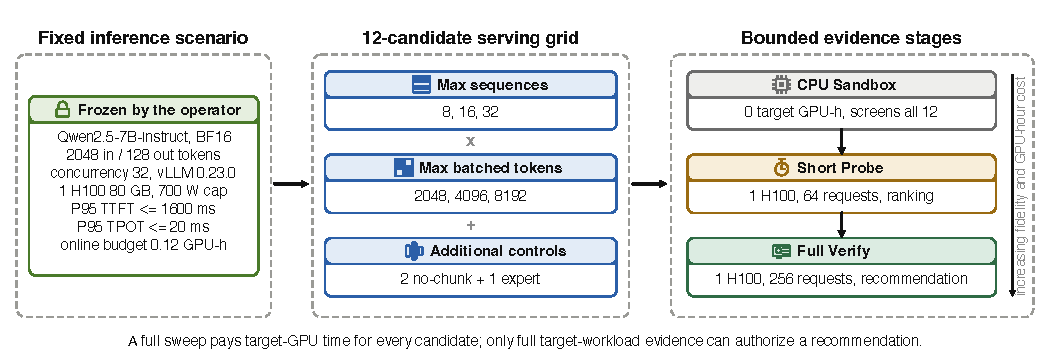
\includegraphics[width=\textwidth]{figures/results/fig1_decision_problem.pdf}
\caption{The bounded single-GPU decision problem.  A frozen model, workload,
SLO, and online budget define 12 immutable serving candidates: nine chunked
combinations from three sequence limits and three batched-token limits, two
no-chunk controls, and one expert default.  A full sweep pays target-GPU cost
for every candidate; \system{} instead screens all candidates in the CPU
Sandbox, escalates selected configurations to a short H100 Probe, and allows a
recommendation only after full target-workload verification.}
\label{fig:motivation}
\end{figure*}


\subsection{Observation 1: Configuration Rankings Are Conditional}

Prefill and decode stress different hardware resources, so a serving knob can
change energy and latency in opposite directions across token geometries.
Continuous batching, chunked prefill, prefix reuse, quantization,
and power policy further alter the realized schedule
\cite{kwon2023vllm,agrawal2024sarathi,zhong2024distserve,lee2026beam}.
Prior energy studies therefore find no universally best
model--engine--workload configuration
\cite{niu2025engines,fernandez2025energy}.  A useful search state must preserve
workload geometry, serving schedule, hardware state, and SLO, rather than reduce a
request to model FLOPs or mean GPU utilization.

\textbf{Requirement R1: scenario-conditioned decisions.}  The controller must
represent the complete deployment scenario and optimize the feasible frontier
for that intent, not learn one global configuration ranking.

\subsection{Observation 2: Cheap Evidence Is Useful but Not Authoritative}

Serving simulators can prune large configuration spaces after small profiling
campaigns \cite{agrawal2024vidur,yang2026charon}.  A single-GPU probe can also
measure prefill, decode, and power response directly.  Neither source observes
the full target run: the CPU model approximates runtime behavior, and a short
probe may not reach the target trace's batching, queueing, and thermal regime.
Prediction uncertainty must therefore grow when a candidate crosses an
unmeasured context, concurrency, serving-policy, or probe-duration boundary.

\textbf{Requirement R2: explicit evidence contracts.}  Every outcome must retain
its stage, provenance, and uncertainty.  A CPU estimate cannot be relabeled as
measured, a short probe cannot be relabeled as the target trace, and a released
recommendation must be supported by full target-workload evidence.

\subsection{Observation 3: Measurement Value Is Decision Dependent}

Uniform sweeps give equal priority to unequal decisions.  A candidate that is
clearly infeasible or dominated does not need a precise target-workload label.
By contrast, a cheap observation can be valuable when it changes the ordering
of two candidates near the frontier, resolves whether an SLO is met, or
calibrates a previously unseen workload or serving regime.  Generic predictive variance is also
insufficient: high uncertainty far from the feasible frontier may have no
effect on the final recommendation.

\textbf{Requirement R3: cost-normalized decision information.}  Acquisition
must jointly select configuration and fidelity according to expected change in
the high-fidelity SLO/Pareto decision per real GPU-hour.

\textbf{Requirement R4: bounded semantic autonomy.}  Natural-language intent,
heterogeneous execution failures, and human escalation benefit from an LLM
planner, but numerical prediction, feasibility, Pareto sorting, budget
accounting, and recommendation release must remain deterministic and auditable.
This separation makes the agent contribution testable against both an
optimizer-only controller and an LLM-only tool user.
